% 第 7 题折线图：按固定源内容流矢量层精确值复刻（1 pt → 0.03515 cm，与全库同制）。
% 原点取坐标系原点 O（源页 (577.9520, 311.5210) pt），y 向上；两轴等比例 28.3468 pt/单位（足尺）。
% 源实测：x 轴 (535.4318,311.5210)→(645.2328,311.5210)（箭头顶点 648.8190）；y 轴竖直 (577.9520,325.6944)→(577.9520,244.2404)（箭头顶点 240.6540）；
% 折线 A(−1,0)→C(0,2)→B(2,0)（单条路径两段、实线、无标记、无刻度短线）；九枚标签照源字形包围盒中心定位。
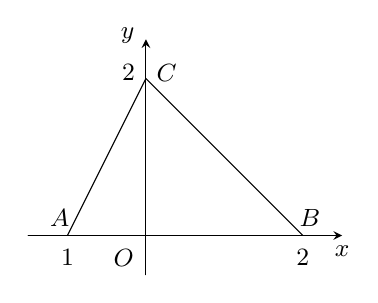
\begin{tikzpicture}[x=0.03515cm,y=0.03515cm,>=stealth,every node/.style={font=\small,inner sep=0pt},
  gl/.style={line width=0.398bp,line cap=round,line join=round}]
% ===== 坐标轴（含箭头，顶点照源实测）=====
\draw[gl,->] (-42.5202,0)--(70.8670,0);   % x 轴
\draw[gl,->] (0,-14.1734)--(0,70.8670);   % y 轴
% ===== 折线 ACB（A(−1,0)→C(0,2)→B(2,0)）=====
\draw[gl] (-28.3468,0)--(0.0002,56.6940)--(56.6932,0);
% ===== 九枚标签（照源字形包围盒中心；斜体字母走数学、数字正体）=====
\node at (-6.6470,72.2510) {\(y\)};
\node at (-6.3270,58.7710) {2};
\node at (7.4530,58.5660) {\(C\)};
\node at (-31.1820,6.3210) {\(A\)};
\node at (59.2680,6.3210) {\(B\)};
\node at (70.8680,-5.5940) {\(x\)};
\node at (-28.3470,-7.8390) {1};
\node at (56.6930,-7.8390) {2};
\node at (-7.9970,-8.2490) {\(O\)};
\end{tikzpicture}
